
\documentclass[12pt,journal,compsoc]{IEEEtran}
\ifCLASSOPTIONcompsoc
\else
\fi
\ifCLASSINFOpdf
\else
\fi
\providecommand{\PSforPDF}[1]{#1}

\usepackage{listings}
\usepackage{graphicx}

\newcommand\MYhyperrefoptions{bookmarks=true,bookmarksnumbered=true,
pdfpagemode={UseOutlines},plainpages=false,pdfpagelabels=true,
colorlinks=true,linkcolor={black},citecolor={black},pagecolor={black},
urlcolor={black},
pdftitle={RSA Cryptosystem Generation of Public and Private Keys in Rust},
pdfsubject={Typesetting},%<!CHANGE!
pdfauthor={Pearson/Demorest},
pdfkeywords={RSA, rust, key generation, large prime numbers}}%<^!CHANGE!


\begin{document}
\lstset{language=bash}
%
% paper title
% can use linebreaks \\ within to get better formatting as desired
\title{RSA Cryptosystem Generation of Public and Private Keys in Rust}
\author{~Dr.~Elise~de Doncker,~Jason~Pearson,~Sam~Demorest% <-this % stops a space
\thanks{}}

% The paper headers
\markboth{}%
{Shell \MakeLowercase{\textit{et al.}}: RSA Cryptosystem Generation of Public and Private Keys in Rust}



\IEEEcompsoctitleabstractindextext{%
\begin{abstract}
	The goal of our project was to develop two programs. The first program would be for determining large prime numbers and the second program for using the first application to create public and private key pairs and using these pairs to encrypt/decrypt a message.
\end{abstract}
\begin{IEEEkeywords}
RSA, rust, key generation, large prime numbers
\end{IEEEkeywords}}


% make the title area
\maketitle

\IEEEdisplaynotcompsoctitleabstractindextext
\IEEEpeerreviewmaketitle



\section{Introduction}
\IEEEPARstart{T}{his} project under the supervision of Dr. Elise de Doncker is to implement the numerous algorithms needed to create a public and private RSA key pair set. 


\section{Research}
At the start of our project we first researched what an RSA key is and how to generate them and discovered it only takes a few steps. The first step is to create two prime numbers. The larger the prime number the better the encryption. Then with these two prime numbers we would be able to create a public and private key. 
\newline \indent We found two algorithms for finding if a number is prime or not. The first is the AKS Primality Test. This primality test is the best deterministic primality test known in terms of time complexity. This being said it is still very slow when compared to non deterministic primality testing algorithms. So we also looked at the Miller Rabin probabilistic primality tests to also test numbers which runs much faster than the AKS primality test.

\section{Design}
First we needed to select a programming language. We both had expressed interest in the new beta programming language Rust and after some research we discovered that it would be a good language to use. Rust is an open-source compiled language that is syntactically similar to C and C++ with an emphasis on control of memory layout and safety.  
\newline
\indent After choosing what language we were going to use the first thing we did was see if someone had already created a primality testing library that we could use. Upon inspecting the algorithms that were available in the libraries on crates.io used the Sieve of Eratosthenes technique. This algorithm calculates all numbers that are less than n that are prime. This is good for if you need small prime numbers, but our goal was to generate large prime numbers. \newline \indent
With no library available we decided that we would have to create our own large prime generator. Because there was no library available we decided to pull that section of code out and create our own library. Once the project is completed that section of code will be publicly available on GitHub under MIT/Apache-2.0 license.


\section{Implementation}
The prime generator used two different primality tests. We used the Miller-Rabin testing for our generation of prime numbers but also implemented the AKS test so we could test both algorithms out.
In the end we decided that AKS was too slow and to stick to the Miller-Rabin primality test.
Before any test was used we made sure the number wasn't even to make sure we aren't using lots of time for easy to find compound numbers.
\newline \indent The key generator calls the prime generation method of the first program and that takes care of all the work for prime number generation. After it gets the prime numbers p and q we use those to compute n which is simply p times q. Next we determine φ(n) which is simply $n - (p + q -1)$. After these are all computed we create a good e value and compute d. The e value is simply a number \\1 $<$ e $<φ(n)$. Then d = e$^{-1}$(mod(φ(n)), which is the private key part of the encryption.


\section{Testing}
Since the two programs were separate we had a rather easy time testing each one out individually. 
For our prime number generator it was fairly simple to determine that our tests are working correctly. All that we had to do was send in some numbers that we know are prime and some that are not prime and make sure that both tests responded accordingly. \\ \indent
To test our program we took an example and tested that our input and output matched. For the example we took some small prime numbers just for testing. So for p and q we took the values 61 and 53 respectively. Then we know that it should calculate for n as 3233 and we know that the totient that it creates should be 3120. For e we need to assign it a value so we can calculate the other values correctly. So for this example we chose 17 and when we calculate the d value we get 2753. \newline \indent
Now using those values we can compute what A should encrypt to and determine if our program is encrypting the value correctly. So the ASCII value of A is 65, so our ciphertext would be ${65}^{17}\mathrm{mod}3233=2790$. So for our test values we know that A should be encrypted to 2790. For testing our decryption part we just have to make sure it calculates 2790 back to A.

\section{Goals Reached}
Our initial goals were to create a primality testing section and to create public and private keys. We were successful in testing for prime numbers with a deterministic method and a non-deterministic method. Another goal of ours was to encrypt and decrypt an input string and we were also successful in this goal. \\ \indent One of our stretch goals was not reached. We were hoping to be able to use our program with other programs that use public and private key pairs such as ssh. We determined this to be out of scope because of the strict standards set up by the IEEE. 

\section{User Guide}
To run this program it is very simple. First you will need to build the program so cd to the directory and run 
%\begin{lstlisting}[frame=single]
cargo build
%\end{lstlisting} 
This compiles the program then to run it we simply do 
%\begin{lstlisting}[frame=single]
cargo run X 
%\end{lstlisting}
Where X is the bit size. The larger the bit size the longer the program will run. After you run the application it will ask for a character you would like encrypted then decrypted. Below is an example run of the program\newline

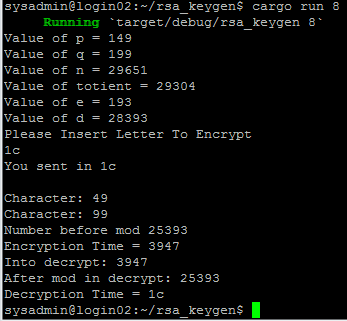
\includegraphics[scale=0.6]{Capture.png}


\section{Conclusion}
The program does generate large prime numbers as it is advertised to do, however with the larger bit sizes the time to calculate a prime number takes a very long time. Keeping in mind that finding a prime number is exponential in terms of complexity it should be understood that there is no better way to do this. The program also can do encryption using different bit sizes, but gets very buggy the larger the bit size. We think that the reason for this issue is due to language that we chose more specifically the BigInt library. However the language is still in its beta phases so as it becomes more developed there will be more support for complex computations. Even with these challenges we were able to create a program that met most of our goals and was able to actually encrypt and decrypt information so we think that the project was successful. 


\end{document}


